% https://github.com/MCG-NKU/NSFC-LaTex
% by Ming-Ming Cheng https://mmcheng.net
% 关于VsCode LaTeX的配置 https://www.cnblogs.com/ourweiguan/p/11785660.html
% Windows下Tex Live最新版可以用pdfLatex快速编译和标准模板相似度更高的文档。



\documentclass[12pt]{article}

\usepackage{cite}
\usepackage{nsfc}
\usepackage{subfig}
\usepackage{cleveref}
\usepackage{float}
% \usepackage{subcaption}

%\usepackage{fontspec}
%\usepackage{xcolor}
%\defaultfontfeatures{Ligatures=TeX}




\newcommand{\addImg}[2][1.0]{\includegraphics[width=#1\linewidth]{#2}}
\newcommand{\cmm}[1]{\textcolor[rgb]{0,0.6,0}{CMM: #1}}
\newcommand{\todo}[1]{{\textcolor{red}{\bf [#1]}}}
\newcommand{\myPara}[1]{\paragraph{#1:}}

\newcommand{\myEmph}[1]{\textbf{\textcolor[rgb]{0,0,0.25}{#1}}}
\newcommand{\mySec}[1]{\vspace{0.15in} \noindent \myEmph{$\square$~#1}}

\graphicspath{{figures/}}



% 设置图形引用的格式  
\crefname{figure}{图}{图} 
\crefname{table}{表}{表} 
\begin{document}




%\if 0
\begin{center}\bf\Large 卫星导航拒止环境下无人机超远距大倾角视觉定位关键技术研究 \\

Research on target recognition *** 
\end{center}





\textbf{摘要}:
%
“用……方法(手段)进行……研究,探索/证明……问题,
对阐明……机制/揭示……规律有重要意义,为……奠定基础/提供……思路 ”。
作用:画龙点睛。
效果:引发评议专家兴趣,使其产生探个究竟的好奇心——“他到底要怎么做?”
摘要字少,但切忌平淡无奇(要勾起评委浓厚兴趣)。
\myEmph{一定要语气坚定,旗帜鲜明,字数有限,资源宝贵,要特别注意重点突出,
讲明现状、意义、课题主要研究目标、内容、思路和预期结果}。



\textbf{Abstract}:
***


科学问题属性:聚焦前沿,独辟蹊径



计算机视觉研究正在经历一个各种检测识别技术大规模进入实际应用的时期。
然而,如何面对绝大多数实际应用中样本数据不足、场景类别不确定、
采集数据质量低等现实问题,
研究不确定环境下小样本目标识别,
依然是计算机视觉领域的世界级科技前沿问题。
%
该问题的解决,有望带领计算机视觉技术进入更为广阔的深水区。
申请人团队拟基于图像场景理解领域内世界前沿的学术成果积累,
在时效性约束和资源受限条件下,研究不确定性的建模及其诱导的
鲁棒深度学习技术,开发适应能力强的神经网络技术,
并利用通用经验知识,推动不确定环境下小样本目标识别理论和方法的突破。
%
相对于现有工作,本项目拟研究的技术具有鲜明的引领性。
不同于传统技术尽量避免不确定性,
该研究计划系统地对不确定性进行建模,并且利用不确定性的特点开发鲁棒的智能算法,
因而,该项目独辟蹊径,有望引领该领域的国际前沿研究发展。


\clearpage
%\fi


%%%%%%%%% TITLE
\title{报告正文}

\maketitle

\emph{\large 参照以下提纲撰写,要求内容翔实、清晰,层次分明,标题突出。
\nsfClr{请勿删除或改动下述提纲标题及括号中的文字。}
}


\ContentDes{(一)立项依据与研究内容(建议$8000$字以下):}


\NsfcSection{1}{项目的立项依据}{
(研究意义、国内外研究现状及发展动态分析,需结合科学研究发展趋势来论述科学意义;
或结合国民经济和社会发展中迫切需要解决的关键科技问题来论述其应用前景。
附主要参考文献目录);}

\subsection{研究背景及科学意义}
在当前全球军事发展趋势下,未来战争与冲突正朝着无人化、智能化的方向加速演进,无人机(Unmanned Aerial Vehicle, UAV)作为关键技术装备,将在未来作战中广泛应用于侦察、打击、通信中继等多个领域。21世纪以来,军用无人机在全球迅速扩散,已在中东、非洲、俄乌冲突等地频繁出现,全球超过80个国家装备了各类军用无人机。在民用领域,随着“低空领域开放”及“加快通航发展”等有利政策的陆续出台,无人机的应用场景不断拓展,已成为推动相关行业智能化和高效化的重要工具。\cite{HKKX201302005}。

\begin{figure}[b]
	\centering
	\subfloat[俄乌冲突中因GNSS干扰被捕获的无人机]{
		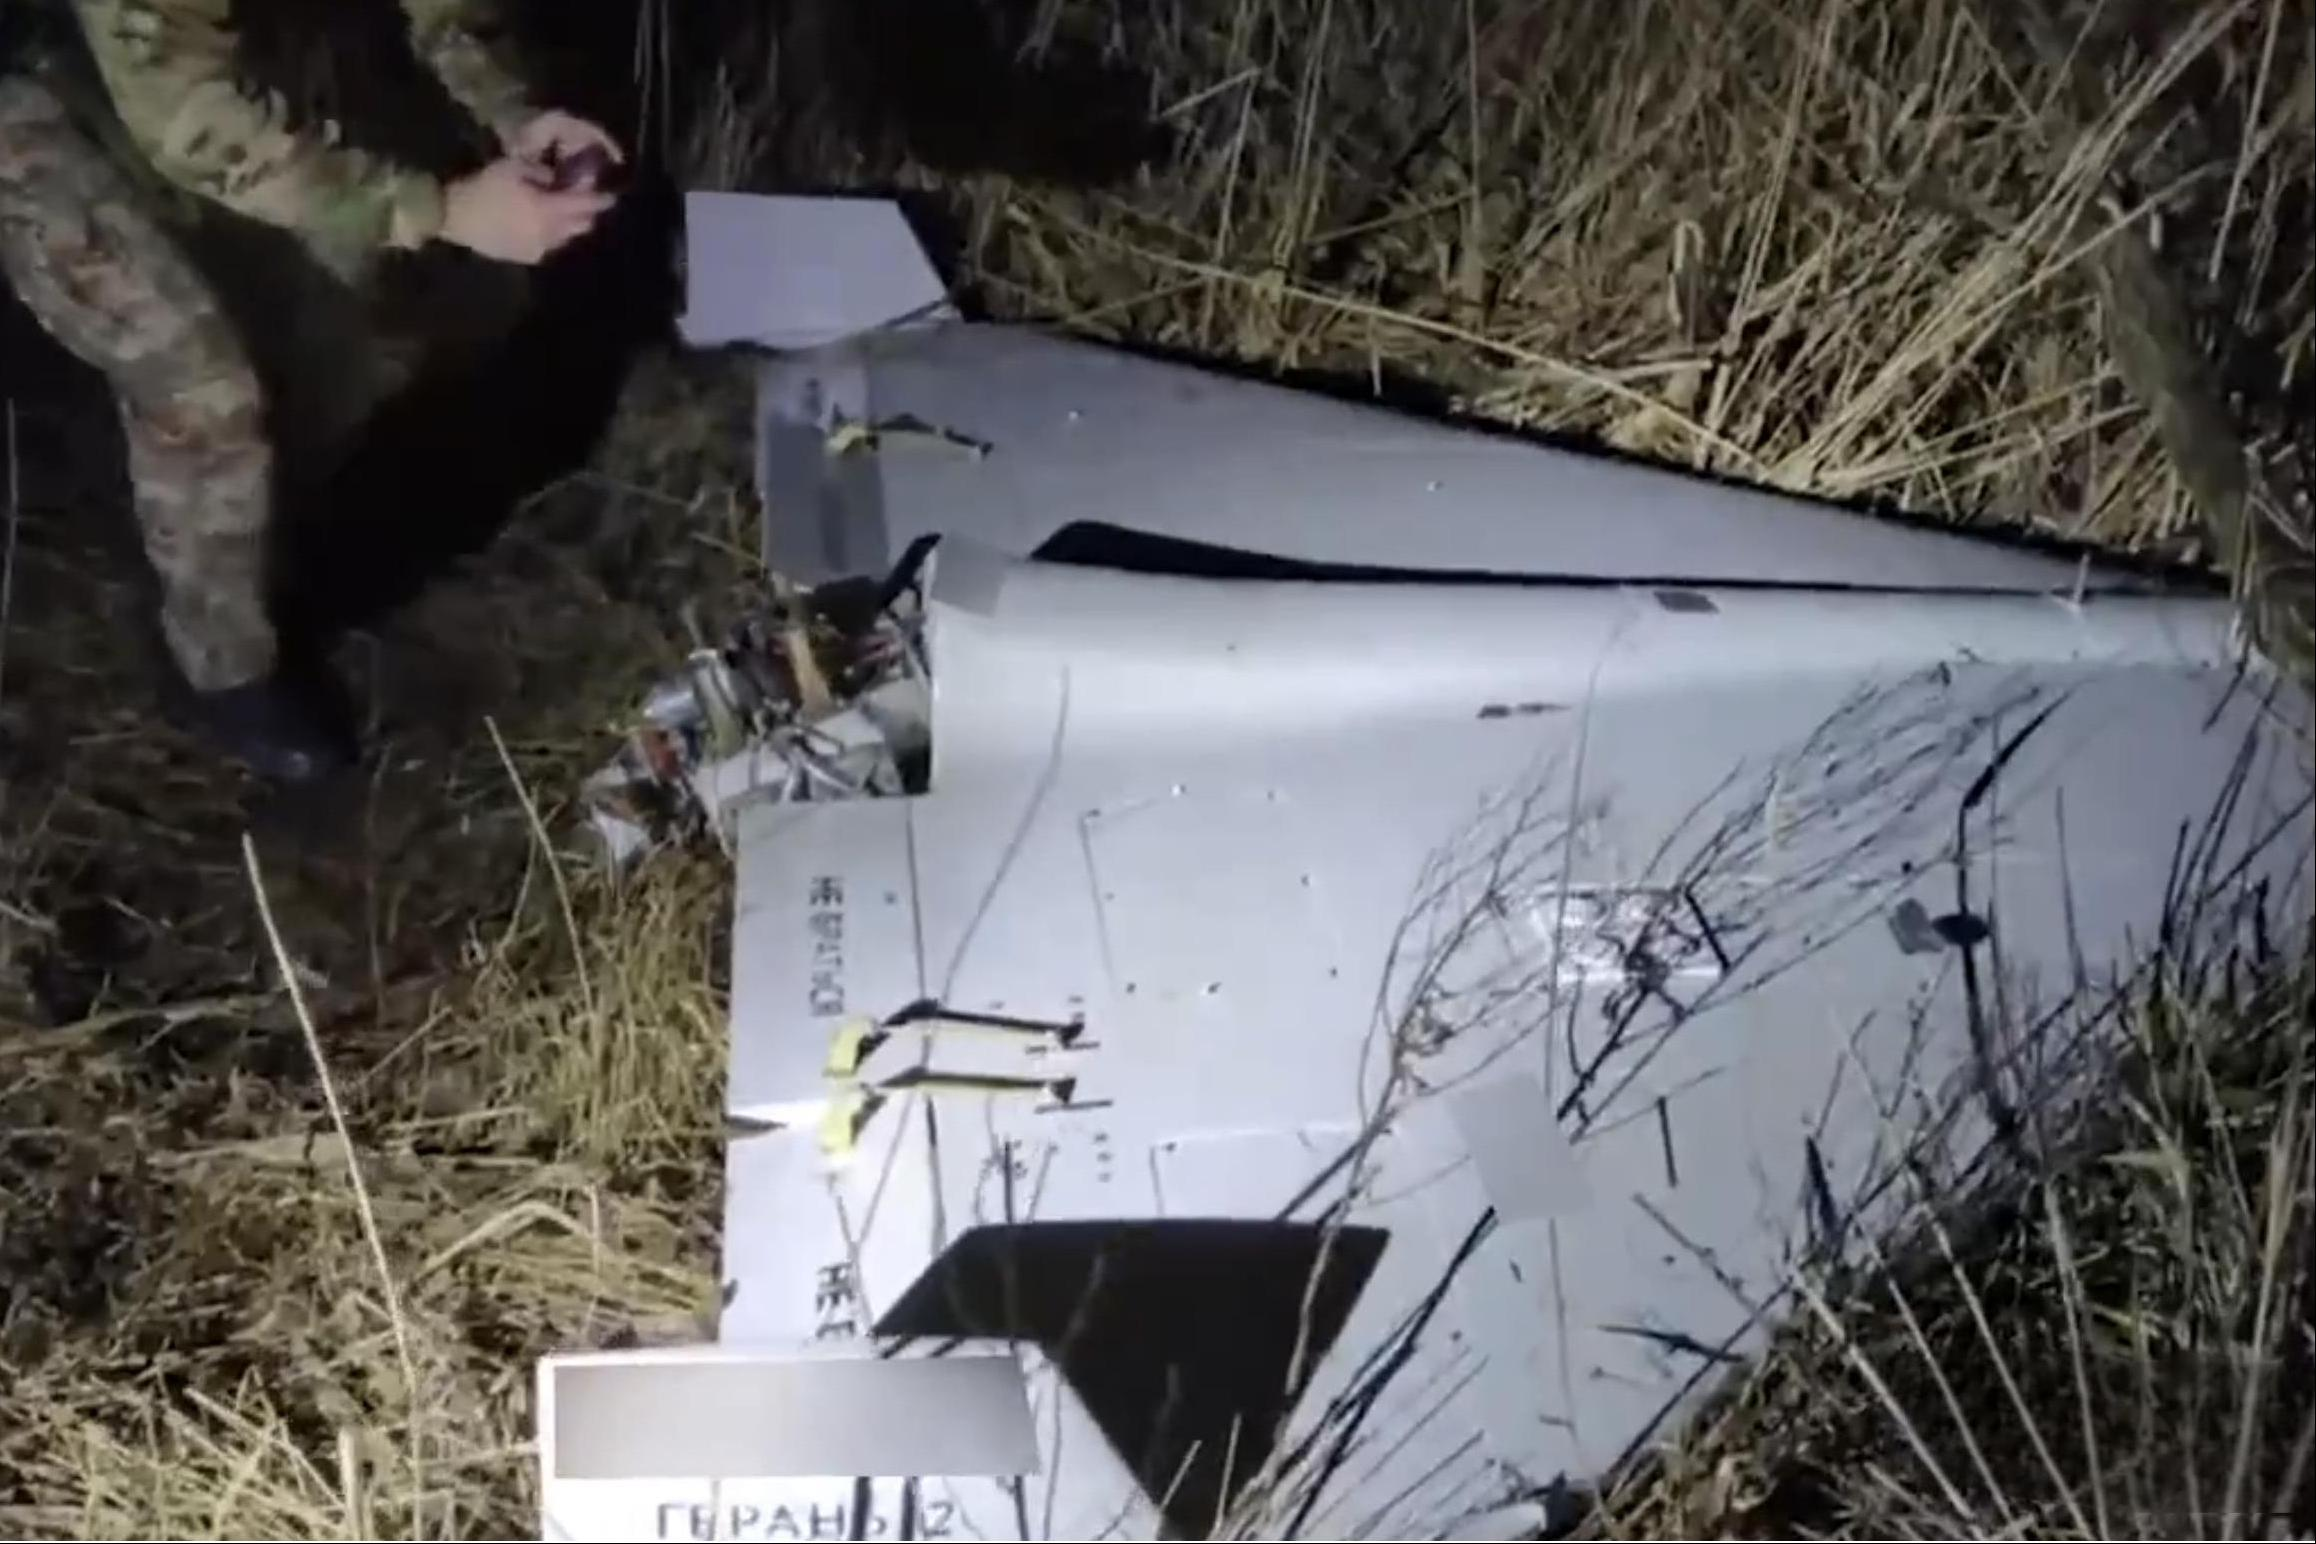
\includegraphics[width=0.48\linewidth]{figures/Pokrova2.jpg}
	} \hfill
	\subfloat[芬航客机因GNSS干扰中止降落塔尔图]{
		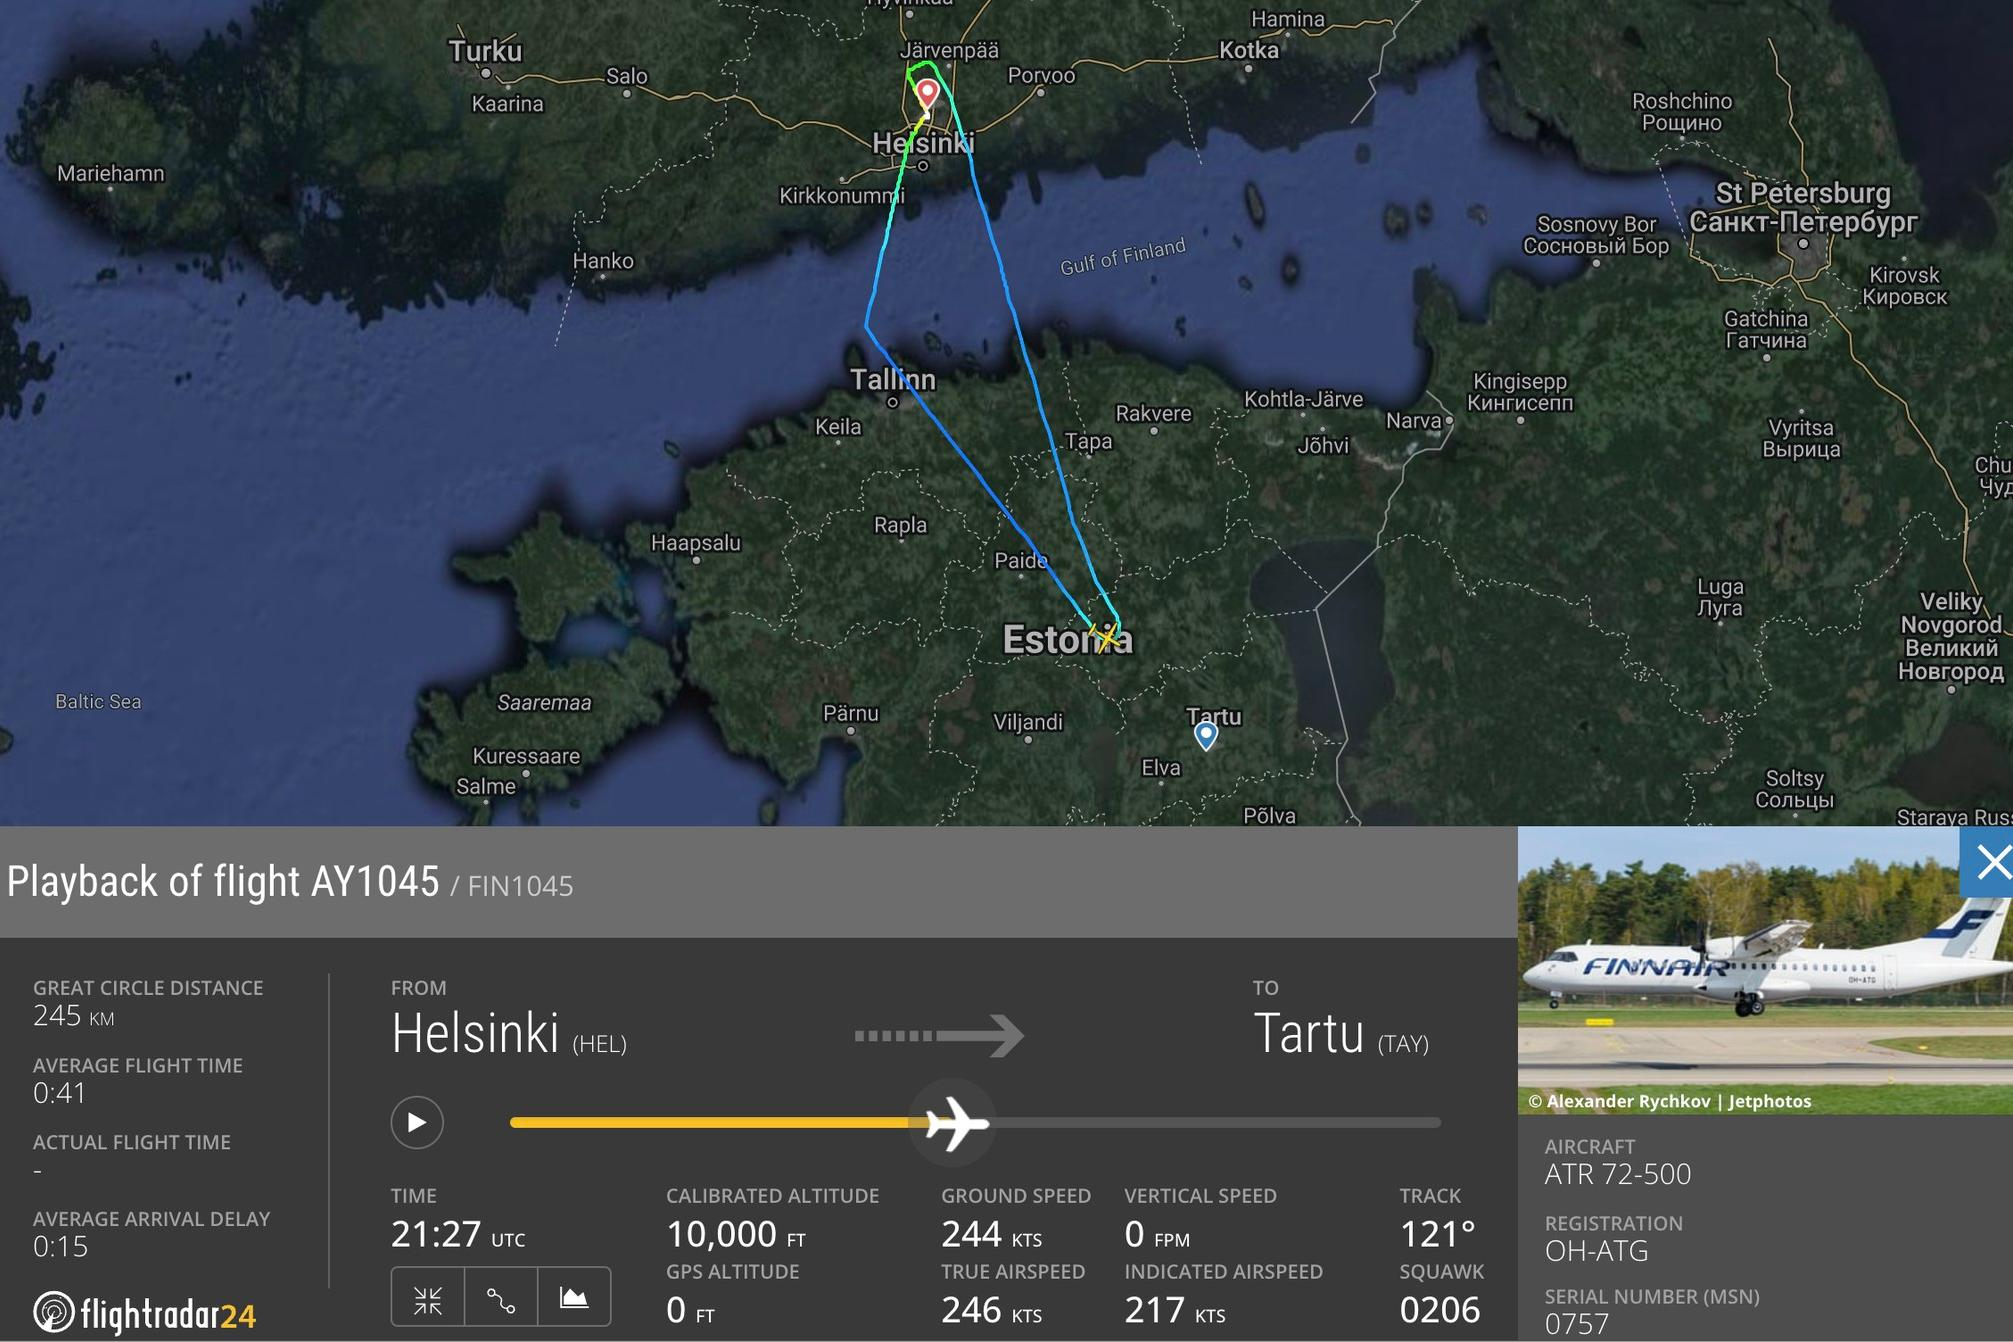
\includegraphics[width=0.48\linewidth]{figures/Finnair.jpg}
	}
	\caption{无人机与民航客机受GNSS干扰案例}
	\label{无人机GNSS欺骗案例}
\end{figure}

然而,当前无论是军用还是民用领域,无人机定位问题的主流解决方案仍高度依赖于全球卫星导航系统(Global Navigation Satellite System, GNSS)。目前在全球范围内广泛应用的GNSS系统包括中国的北斗(BeiDou)、美国的全球定位系统(Global Positioning System, GPS)、俄罗斯的Glonass以及欧洲的Galileo。然而,近年来GNSS系统受干扰的情况日益频发\cite{ZGHT201507010},\Cref{无人机GNSS欺骗案例}展示了GNSS受到干扰的典型案例。\Cref{无人机GNSS欺骗案例}(a)展示了俄乌冲突中因GNSS干扰而被捕获的无人机,GNSS干扰能够通过伪造或阻断卫星信号,使无人机失去导航能力,进而被敌方捕获或控制。\Cref{无人机GNSS欺骗案例}(b)则展示了芬兰航空公司的客机因GNSS干扰而被迫中止在塔尔图机场的降落。这进一步说明,GNSS干扰不仅影响军事行动,还可能对民用航空安全构成严重威胁。


在实际应用中,如\Cref{noGNSS}所示,GNSS信号的干扰或者拒止问题往往由多种因素共同作用。首先,物理遮挡是导致GNSS信号丢失的常见原因之一\cite{BJHK202004019}。无人机在城市峡谷、密集森林或地下隧道等复杂环境中飞行时,建筑物、树木或地形特征会阻挡卫星信号的传输,导致定位精度下降甚至完全失效。其次,人为的电子干扰和压制手段也在不断增加。敌对势力或非法组织可能通过发射强电磁信号,干扰或压制GNSS信号的接收,使得无人机无法准确获取定位信息。此外,GNSS信号还可能受到自然环境的干扰,例如太阳活动引起的电离层扰动,或者极端天气条件下的信号衰减。这些因素共同作用,使得无人机在GNSS拒止环境中的导航和定位面临巨大挑战。

\begin{figure}[t]
	\centering
	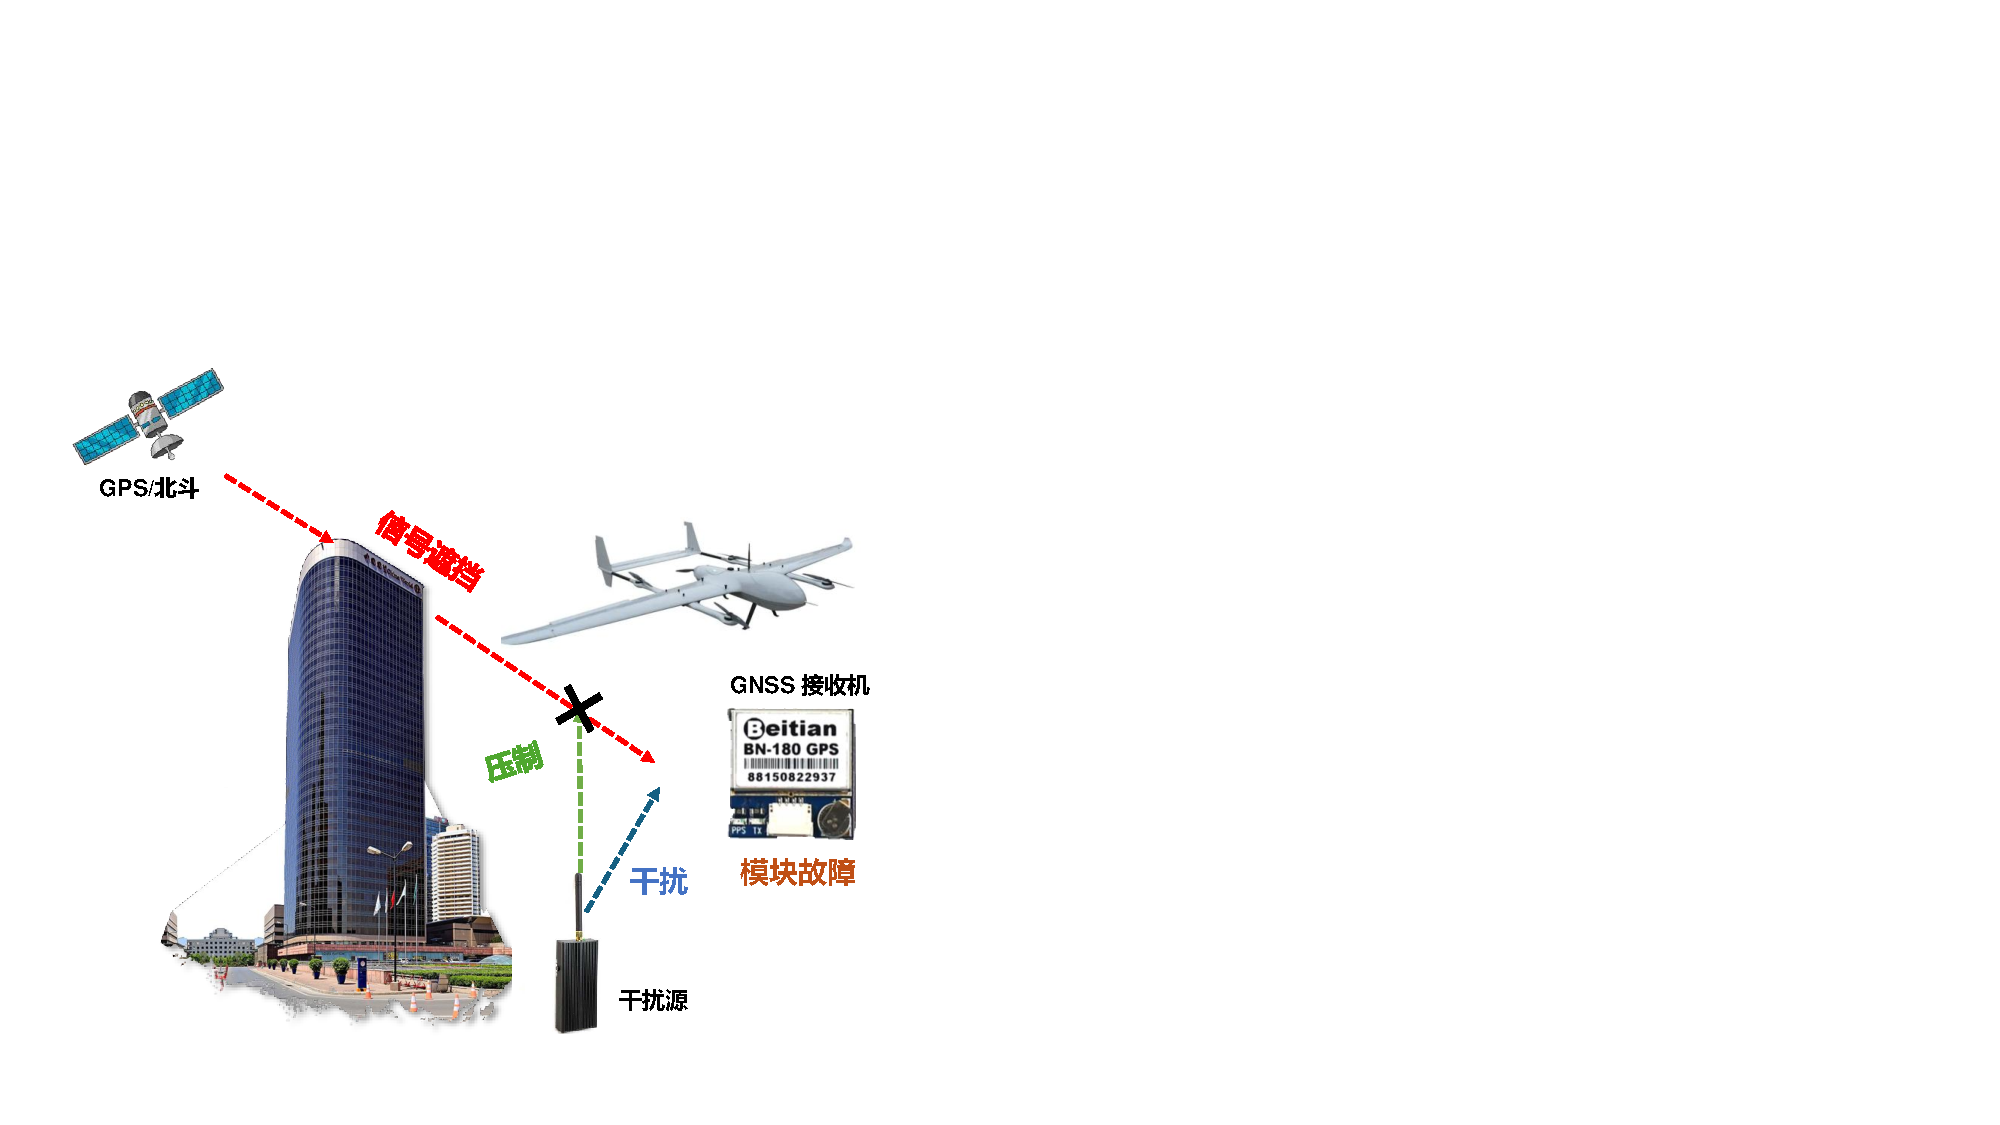
\includegraphics[width=0.8\linewidth]{figures//GNSS拒止示意图.pdf}
	\caption{无人机卫星导航信号拒止示意图}
	\label{noGNSS}
\end{figure}

如\Cref{GNSSregion}所示,2025年1月15日热点区域的GNSS干扰情况揭示了显著的信号干扰现象,全球重点区域的GNSS导航信号干扰对军事领域中的无人机作战效能与任务执行能力构成了重大威胁。无人机在精确导航和定位方面对GNSS系统具有高度依赖性,因此一旦遭遇信号干扰,其定位精度将显著下降,甚至可能完全丧失导航能力。这不仅直接危及无人机的飞行安全,还会严重影响其在侦察、打击以及通信中继等任务中的执行效果。此外,敌方还可能利用信号干扰诱使无人机偏离预定航线,或将其引导进入敌方控制区域,从而导致严重的战术失误和装备损失。因此,研究可靠的备份导航系统已成为提升无人机作战能力和确保任务成功的关键研究方向。


\begin{figure}[H]
	\centering
	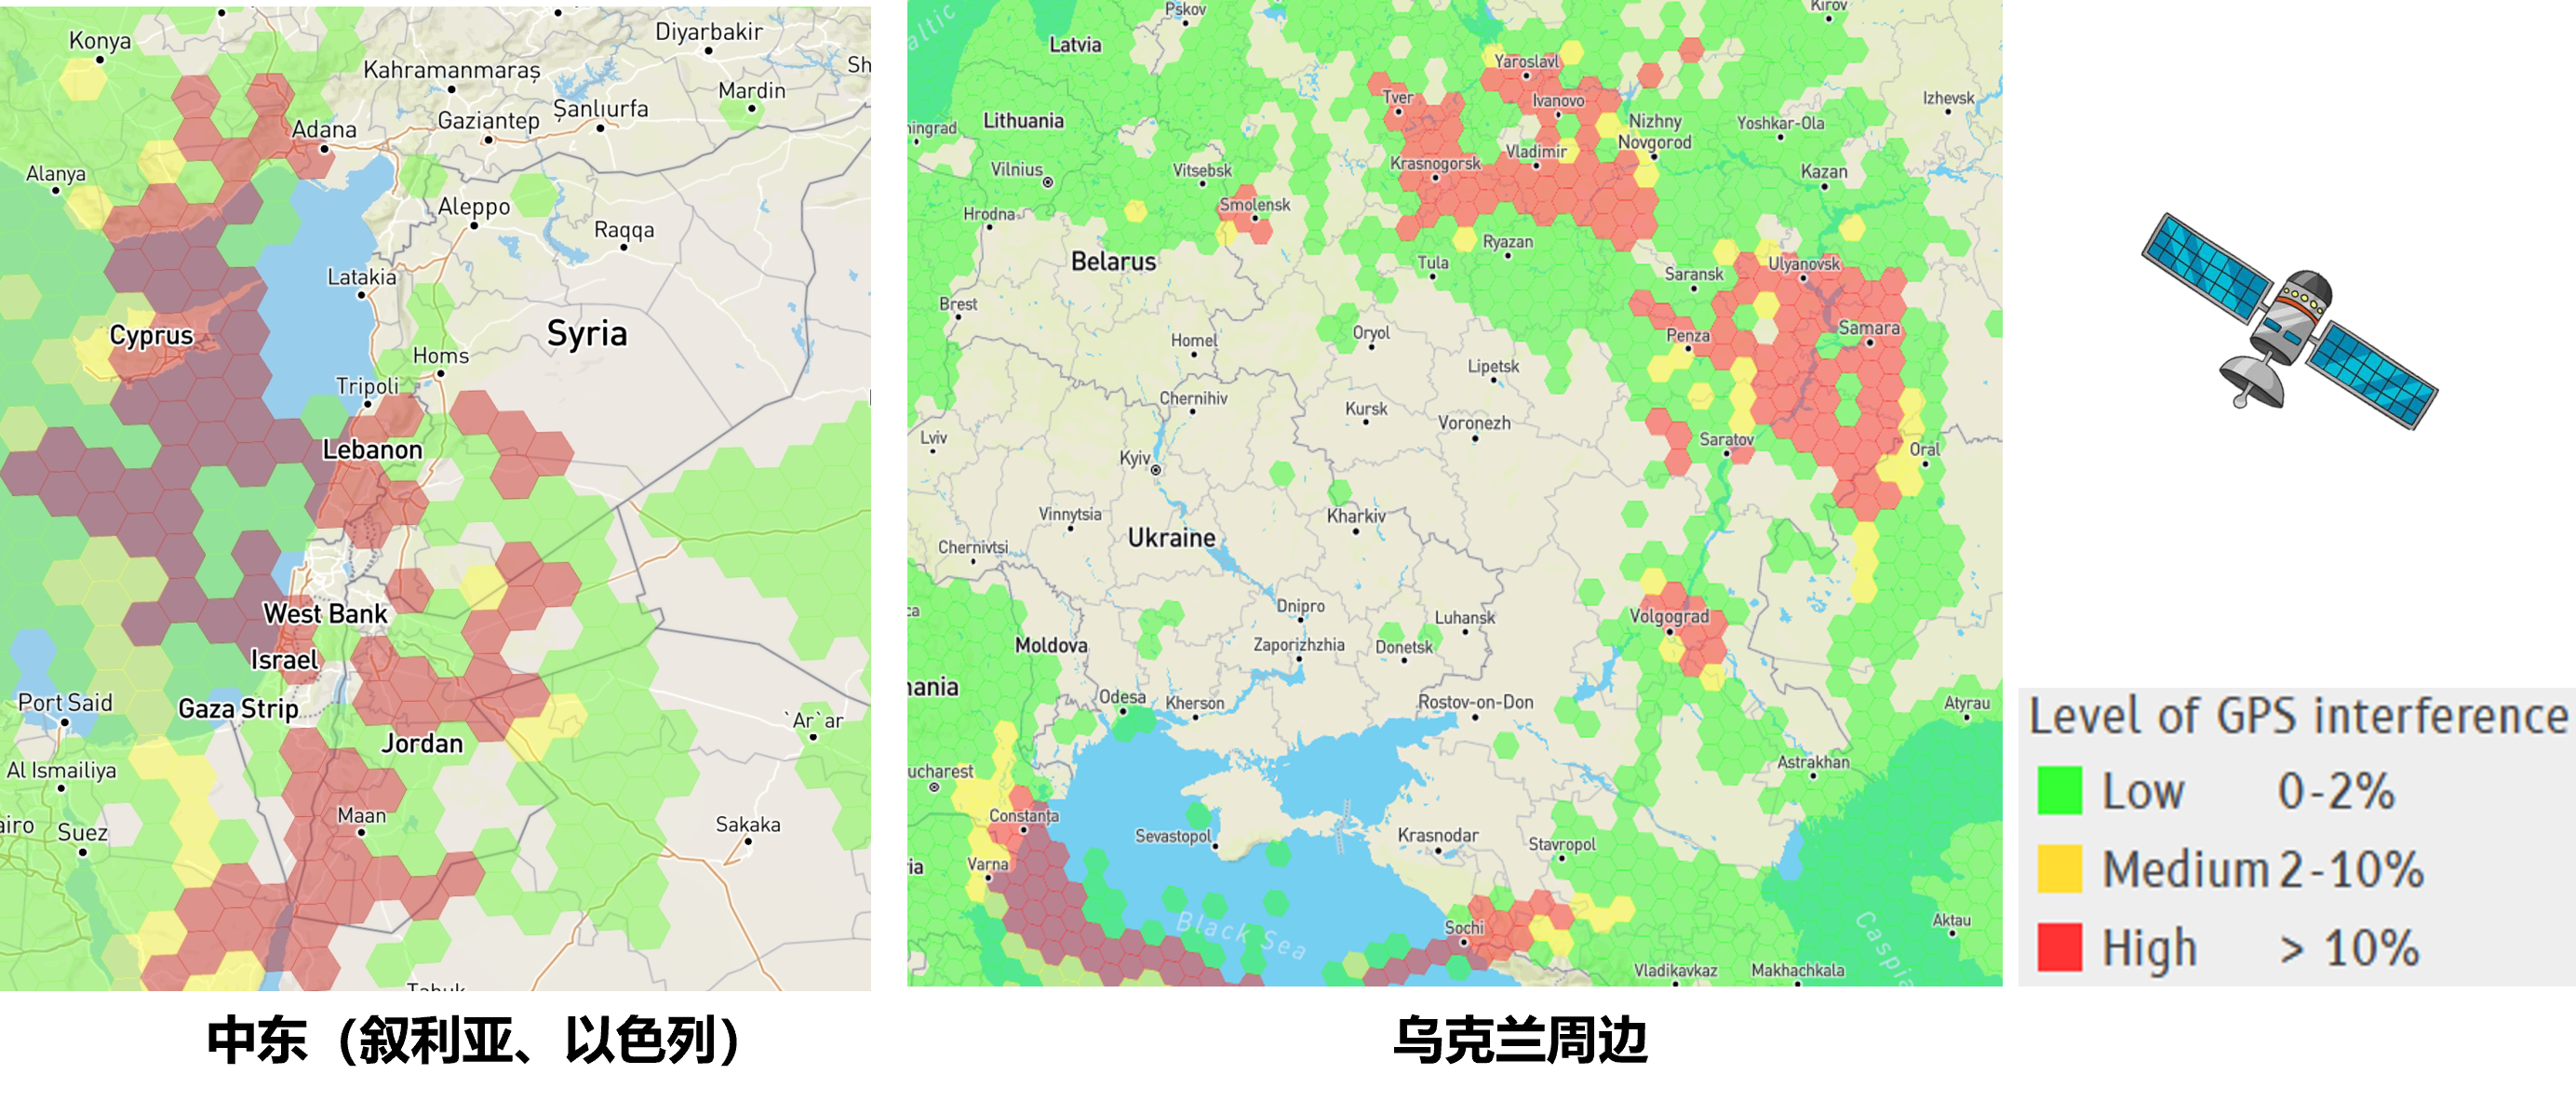
\includegraphics[width=\linewidth]{figures/热点区域GPS干扰情况.png}
	\caption{热点区域GNSS干扰情况(2025年1月15日)}
    \label{GNSSregion}
\end{figure}

各国都纷纷针对GNSS拒止环境的导航技术研究开展研究\cite{CODE},美军围绕GNSS拒止环境下的机载导航、无人作战以及精确武器制导等方面开展了诸多研究。例如,美国国防部高级研究计划局 (Defense Advanced Research Projects Agency,DARPA) 的“拒止环境中协同作战 (Collaborative Operations in Denied Environment,CODE)”项目,旨在提升无人集群在GNSS拒止时的作战能力;DARPA与美国空军研究实验室共同推进的SECTR计划,则致力于改进在GNSS拒止环境下对目标的识别与定位。以色列导航解决方案公司Grupo Oesía推出的GNSS拒止环境导航套件,利用视觉技术实现精确的姿态与位置估计,可有效抵御GNSS“欺骗”和“干扰”威胁。此外,由Archangel Imaging、UAVaid和Novit AI组成的财团已为英国国家航空航天技术开发计划的GENIE项目 (GNSS Excluded Navigation Intelligent Enhancement) 提供资金支持,专注开发适用于GNSS拒止或干扰环境的创新型飞机导航技术。

现有的GNSS拒止环境下的替代性定位技术可分为以下几类,包括地磁定位、星光定位、地形等高线匹配、惯性导航以及基于卫星图像匹配的方法\cite{MOTO202502004}。地磁定位通过精确测量局部磁场的强度矢量即可建立磁场特征与地理位置之间的对应关系,但其精度受限于磁场分布的复杂性和局部磁场的动态变化;星光定位技术则是一种基于天体运行规律的自主导航方法,通过观测天体在天空中的方位角和高度角,结合飞行器的实时姿态信息,可准确推算其三维空间位置,但该技术仅适用于深空探测的飞行器导航;地形等高线匹配技术通过将飞行器实测地形剖面与预存数字地形模型进行相关性匹配从而用于导航,但在平坦或地形特征不明显的区域,匹配效果较差,定位精度无法保证。惯性导航则是一种基于加速度计和陀螺仪测量的航位推算技术,但其劣势在于误差会随时间累积,长期定位精度逐渐下降。基于卫星图像匹配的方法的基本原理是将无人机实时拍摄的图像与卫星影像进行特征匹配,求解两张图像之间的相对位置关系,如\Cref{basicprinciples}所示。由于卫星图像天然携带地理位置坐标(如经纬度信息)\cite{CUXI202410035},通过这种匹配关系,可以进一步推导出无人机的精准定位。总结而言,与上述方法相比,本文提出的卫星影像匹配方法具有以下显著优势:

\begin{figure}
	\centering
	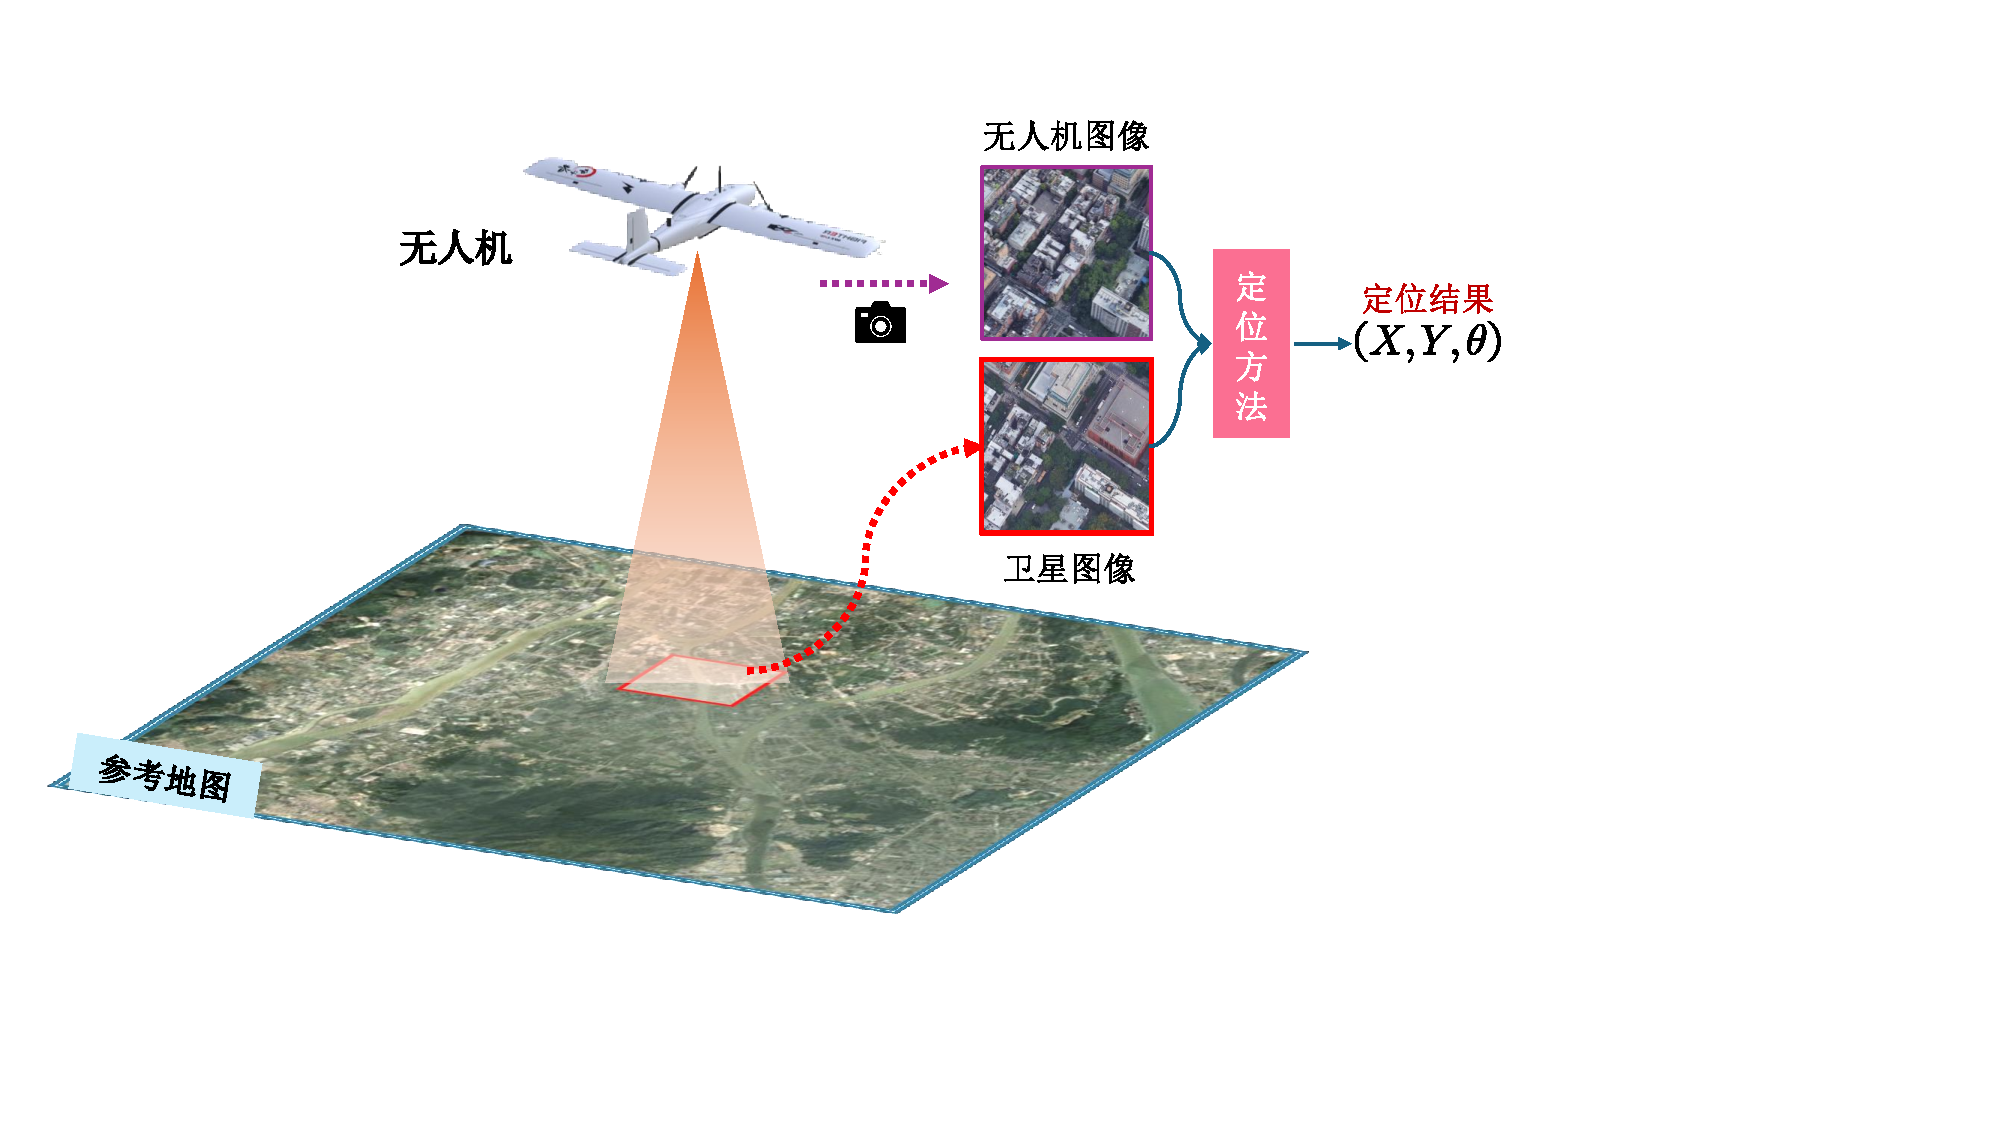
\includegraphics[width=1.0\linewidth]{figures/基于卫星影像匹配的无人机定位示意图2.pdf}
	\caption{基于卫星影像匹配的无人机视觉定位示意图}
 \label{basicprinciples}
\end{figure}

(1)抗电磁干扰能力强。与地磁定位受磁场动态变化影响不同,卫星影像匹配方法不依赖于环境的物理特性,而是基于图像特征的匹配,因而对外界环境变化(如磁场干扰、电磁信号屏蔽等)具有较强的抗干扰能力。(2)低成本且高效能。与依赖高精度传感器的技术(如星光导航和地磁导航)相比,由于无人机通常已配备吊舱等图像采集设备,因此无需增加额外硬件即可实现对应功能,从而显著降低了硬件成本。(3)累计误差相对较小。与惯性导航系统相比,卫星影像匹配技术有效避免了持续累积误差问题,能够提供更为精确和可靠的定位信息,特别适合长时间与长距离的导航任务。

综上所述,基于卫星影像匹配的无人机定位技术凭借其抗电磁干扰能力强、硬件成本低且无累计误差等优势,为解决GNSS拒止环境下的定位问题提供了创新性解决方案。
本研究着眼于这一新形势下无人智能作战的关键技术,紧密围绕军民两用领域的重大战略需求,重点探究基于卫星影像匹配的无人机视觉定位方法。旨在显著提升无人机在复杂环境中的卫星影像匹配精度与速度,不仅可为无人机在应急救援、地理测绘等民用场景提供可靠定位保障,更可拓展至复杂战场环境下的无人系统自主导航,具有显著的军民两用价值。


\subsection{国内外相关工作}

国内外学者针对基于卫星影像的无人机视觉定位方法开展了广泛研究,主要方法可归纳为基于模板匹配、基于局部不变特征点匹配以及基于深度学习的三类方法。其中,基于模板匹配和基于局部不变特征点匹配的方法大多以可见光影像为主。近年来,随着深度学习在特征提取方面的强大能力逐步显现,基于深度学习的视觉定位方法开始逐渐成为研究热点,并根据传感器类型的不同进一步细分为基于可见光、红外热成像和矢量地图的视觉定位方法。以下将对这些方法进行详细分类与讨论。

\textbf{(1)基于模板匹配的视觉定位方法}

模板匹配(Template Matching)作为图像处理与图像匹配领域中的基础技术之一,在图像配准与视觉定位中具有重要作用,亦被称为直接匹配或密集匹配。该方法的核心原理是通过对源图像与模板图像进行逐像素比较,从而识别出最相似的区域,并基于像素级对应关系实现图像的几何对齐,如\cref{relatedwork_image3}所示。



 \begin{figure}[H]
  \centering
  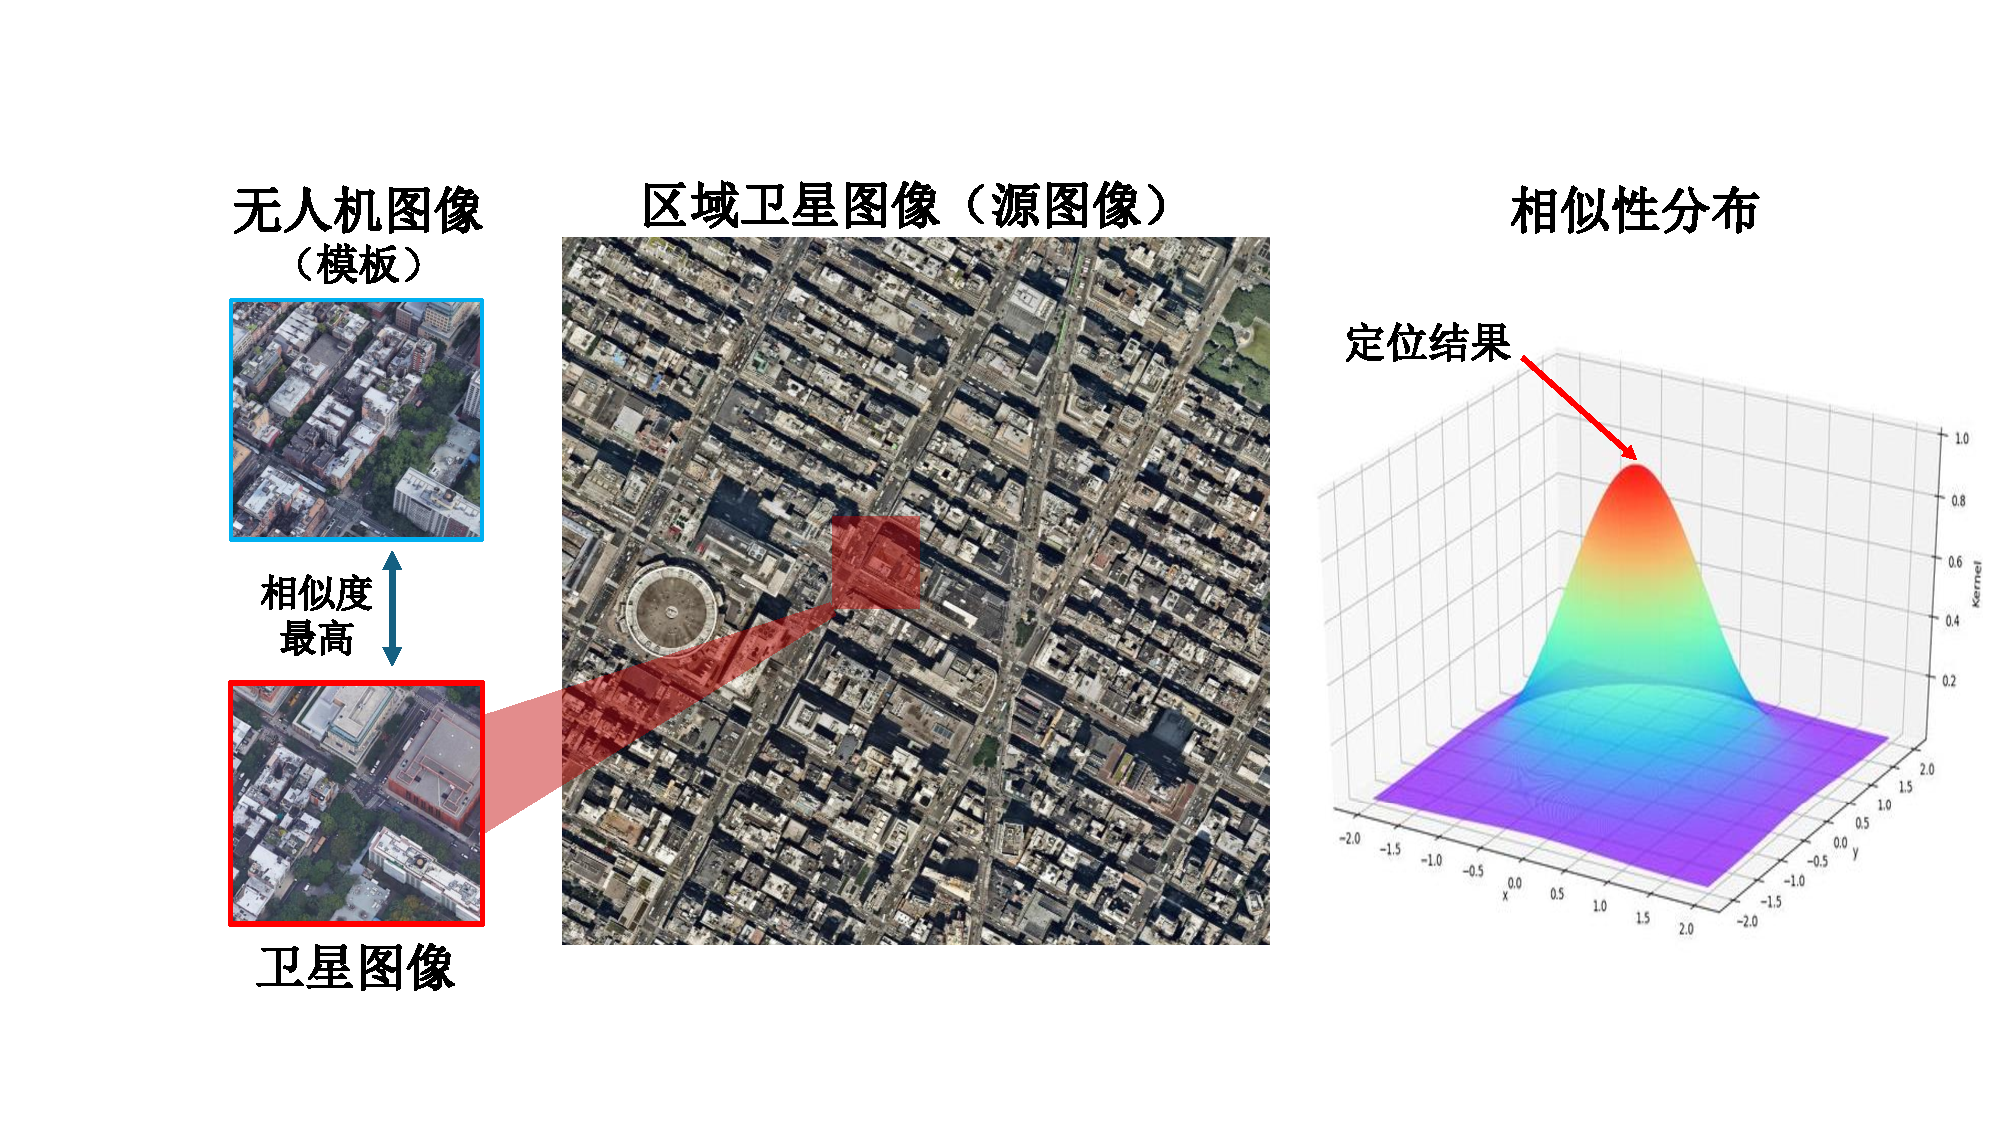
\includegraphics[width=0.9\linewidth]{figures/relatedwork/基于模版匹配的定位方法.pdf}
  \caption{基于模板匹配的视觉定位方法示意图}
  \label{relatedwork_image3}
\end{figure}

{
\bibliographystyle{nsfc.bst}
\bibliography{thesis_ref}
}


%%%%%%%%%%%%%%%%%%%%%%%%%%%%%%%%%%%%%%%%%%%%%%%%%
\NsfcSection{2}{项目的研究内容、研究目标,以及拟解决的关键科学问题}{
(此部分为重点阐述内容);}

\subsection{研究目标}


重点阐述本项目计划\myEmph{做到什么程度}。
一定要用大同行能够理解的术语来描述。

\myEmph{(1)定性研究目标}


\myEmph{(2)定量研究目标}

1.构建一套基于无人机-卫星图像匹配的目标定位模型,在机载处理器Jetson AGX Orin搭载卫星数据库,当数据库规模为1万张时,特征维度为512维时,无人机向量卫星特征向量的相似度度量平均时间不大于0.01秒;

2、粗略检索阶段,当卫星图像数据库为1万张时,在机载处理器Jetson AGX Orin上模型推理平均时间不大于0.05秒;精确定位阶段,单张无人机图与卫星图像的匹配时,模型推理平均时间不大于0.2秒;

3、在公开的无人机-卫星跨视角建筑物检索数据集University1652上(包含多个视角、不同高度),平均检索精度不低于80%;

4、在公开的ALTO数据集上,飞行距离4千米,飞行高度为500±50米,平均定位精度优于50米。


\subsection{研究内容}

本项目针对卫星拒止环境下无人机如何对地面目标进行精确定位问题展开研究,主要的研究内容如图2-1所示,具体包含如下几个方面:梳理卫星拒止环境下无人机对地面目标精确定位需求,构建基于无人机-卫星图像匹配的地面目标定位模型,研究无人机-卫星多视角图像检索与匹配的目标定位方法,最后构建原型系统,开展面向典型应用场景的实验验证。


重点阐述本项目计划\myEmph{做什么}。
如\figref{fig:teaser}所示,建议撰写之前仔细画一个主要研究内容的图。
我通常习惯用PowerPoint作图,做好后导出为pdf格式,既可以保持图片不会文件太大,也可以保证放大后非常清晰。
幻灯片直接导出的pdf可能存在空白边,可以用WPS中的“页面-剪裁页面”去掉白边。
作图用的pptx文件我也通常会保存起来,例如这个模版\LaTeX 文件中的“prepare/NSFC-Figs.pptx”。
如果是大的国基金项目,后续可能涉及答辩。
答辩时这个图可以用,保留pptx格式也方便到时候做尺寸和布局的调整。


\begin{figure}[ht]
	\centering
    \begin{overpic}[width=0.8\columnwidth]{framework.pdf}
    \end{overpic}
    \caption{本项目主要研究内容。
    }\label{fig:teaser}
\end{figure}




\subsection{拟解决的关键科学问题}



\NsfcSection{3}{拟采取的研究方案及可行性分析}{
(包括研究方法、技术路线、实验手段、关键技术等说明);}


\subsection{拟采取的技术路线}

根据拟定的总体研究方案,本课题拟使用的关键技术路线概括为以下四个方面,如图\figref{fig:pipline}所示,:


\begin{figure}[ht]
	\centering
    \begin{overpic}[width=\columnwidth]{pipeline.pdf}
    \end{overpic}
    \caption{本项目的技术路线。
    }\label{fig:pipline}
\end{figure}

\myEmph{(1)基于矢量地图的无人机视觉地理定位方法}

此类传统基于可见光卫星地图的视觉定位方法虽有一定成效,但面临数据采集成本高、存储开销大、易受季节变化影响等瓶颈。相比之下,矢量地图以几何拓扑关系为核心,具备存储效率高、可增量更新、跨季节鲁棒性强等优势,更贴近人类利用简略地图导航的机制。受此启发,本章将第三章的跨模态匹配方法由“红外图像-可见光地图”的匹配扩展到“可见光图像-矢量地图”的匹配,提出VecMapLocNet(Vector Map-Based Visual Localization Network)视觉定位方法,将矢量地图引入无人机视觉定位任务,通过跨模态匹配实现无人机3自由度位姿(纬度、经度、航向角)的精准估计。具体而言,VecMapLocNet基于端到端架构设计,包含三大核心模块:(1)无人机图像编码模块采用轻量化多尺度特征提取网络,通过残差连接与跨层融合机制,有效应对飞行高度变化引起的尺度差异,同时适配边缘计算设备的低延迟需求;(2)提出一种加权矢量地图编码模块MapVectorizer,借鉴大语言模型的语义加权思想,对矢量地图进行自适应特征编码,动态区分建筑物、道路等关键地标与次要元素的贡献权重,显著提升跨模态匹配的判别性;(3)位姿估计模块基于傅里叶变换的旋转模板匹配策略,通过频域相关性计算与逆变换生成概率图,实现无参数化、高效率的3自由度位姿解算。此外,系统引入旋转增强与多尺度对齐机制,进一步增强了复杂视角与动态环境下的鲁棒性。

\subsection{可行性分析}

既然国内外相关工作都没能解决你提出的重要问题,为什么你觉得自己有望解决该问题。
论述的时候通常包括:独特的时机、与众不同的方案、雄厚的相关科研积累等。


\NsfcSection{4}{本项目的特色与创新之处;}{}

您的方法有什么独特性,为什么您认为它会成功?

\NsfcSection{5}{年度研究计划及预期研究结果}{
(包括拟组织的重要学术交流活动、国际合作与交流计划等)。}

\subsection{年度研究计划}
本课题组对研究内容进行了充分的预研究,全部研究内容将在4年内完成, 具体计划安排如下:

\subsection{预期研究成果}


(1) \myEmph{形成一套无人机视觉定位应用解决方案}。本项目以\myEmph{“以能实际应用作为最高导向}“需求牵引,突破瓶颈”作为,因此,解决卫星导航拒止环境下无人机视觉定位的实际需求为核心目标,力求突破现有技术瓶颈,研发出具有高精度、高鲁棒性和高实时性的视觉定位算法与系统。研究成果将直接服务于无人机在复杂环境中的自主导航与任务执行能力,推动无人机技术在国防安全、应急救援、精准农业等领域的广泛应用。

(2) \myEmph{取得具有创新性的理论成果}。


(4) \myEmph{培养高素质的科研人才队伍}:


项目各阶段,特别是中期和期末,如何检查该项目计划成功与否?

%%%%%%%%%%%%%%%%%%%%%%%%%%%%%%%%%%%%%%%%%%%%%%%%%
\ContentDes{(二)研究基础与工作条件}


\NsfcSection{1}{研究基础}{
(与本项目相关的研究工作积累和已取得的研究工作成绩);}

申请人在与本项目相关的研究工作中有着丰富的理论基础与工程经验,并取得了国际领先的科研成果, 
发表\myEmph{10余篇CCF A类}国际期刊及会议论文(ACM TOG 4篇,IEEE TPAMI 2篇,
IEEE CVPR 3篇,IEEE ICCV 2篇,IEEE TVCG 2篇),
\myEmph{论文Google Scholar他引450+次,论文单篇最高他引272次}。
这些研究基础主要包括3个方面:

% 申请人在与本项目相关的研究工作中有着丰富的积累,并取得了国际领先的科研成果, 
% 发表\myEmph{10余篇CCF A类}国际期刊及会议论文(ACM TOG 4篇,IEEE TPAMI 2篇,
% IEEE CVPR 3篇,IEEE ICCV 2篇,IEEE TVCG 2篇),
% \myEmph{论文Google Scholar他引1600+次,一作论文单篇最高他引700+次}。
% 这些研究基础主要包括3个方面:


\subsection{基于连续序列匹配的无人机视觉地理定位方法}


在复杂的地理空间场景中,普遍存在视觉特征高度相似的挑战性现象,例如重复的建筑群布局和复杂的道路网络结构等,这些因素对基于视觉特征的定位方法提出了严峻的技术考验。现有方法着眼于孤立的单帧图像,这种一对多的全局匹配方法在处理具有高度相似性的视觉场景时,仍难以有效解决定位过程中出现的歧义性问题。针对这一技术瓶颈,本研究提出了一种连续序列匹配的无人机视觉地理定位框架,如\Cref{seqoverall}所示,该框架充分结合地理空间中的固有约束信息,特别是利用前后帧序列的时间连续性特征,实现了定位精度的显著提升。

\begin{figure}[H]
	\centering
	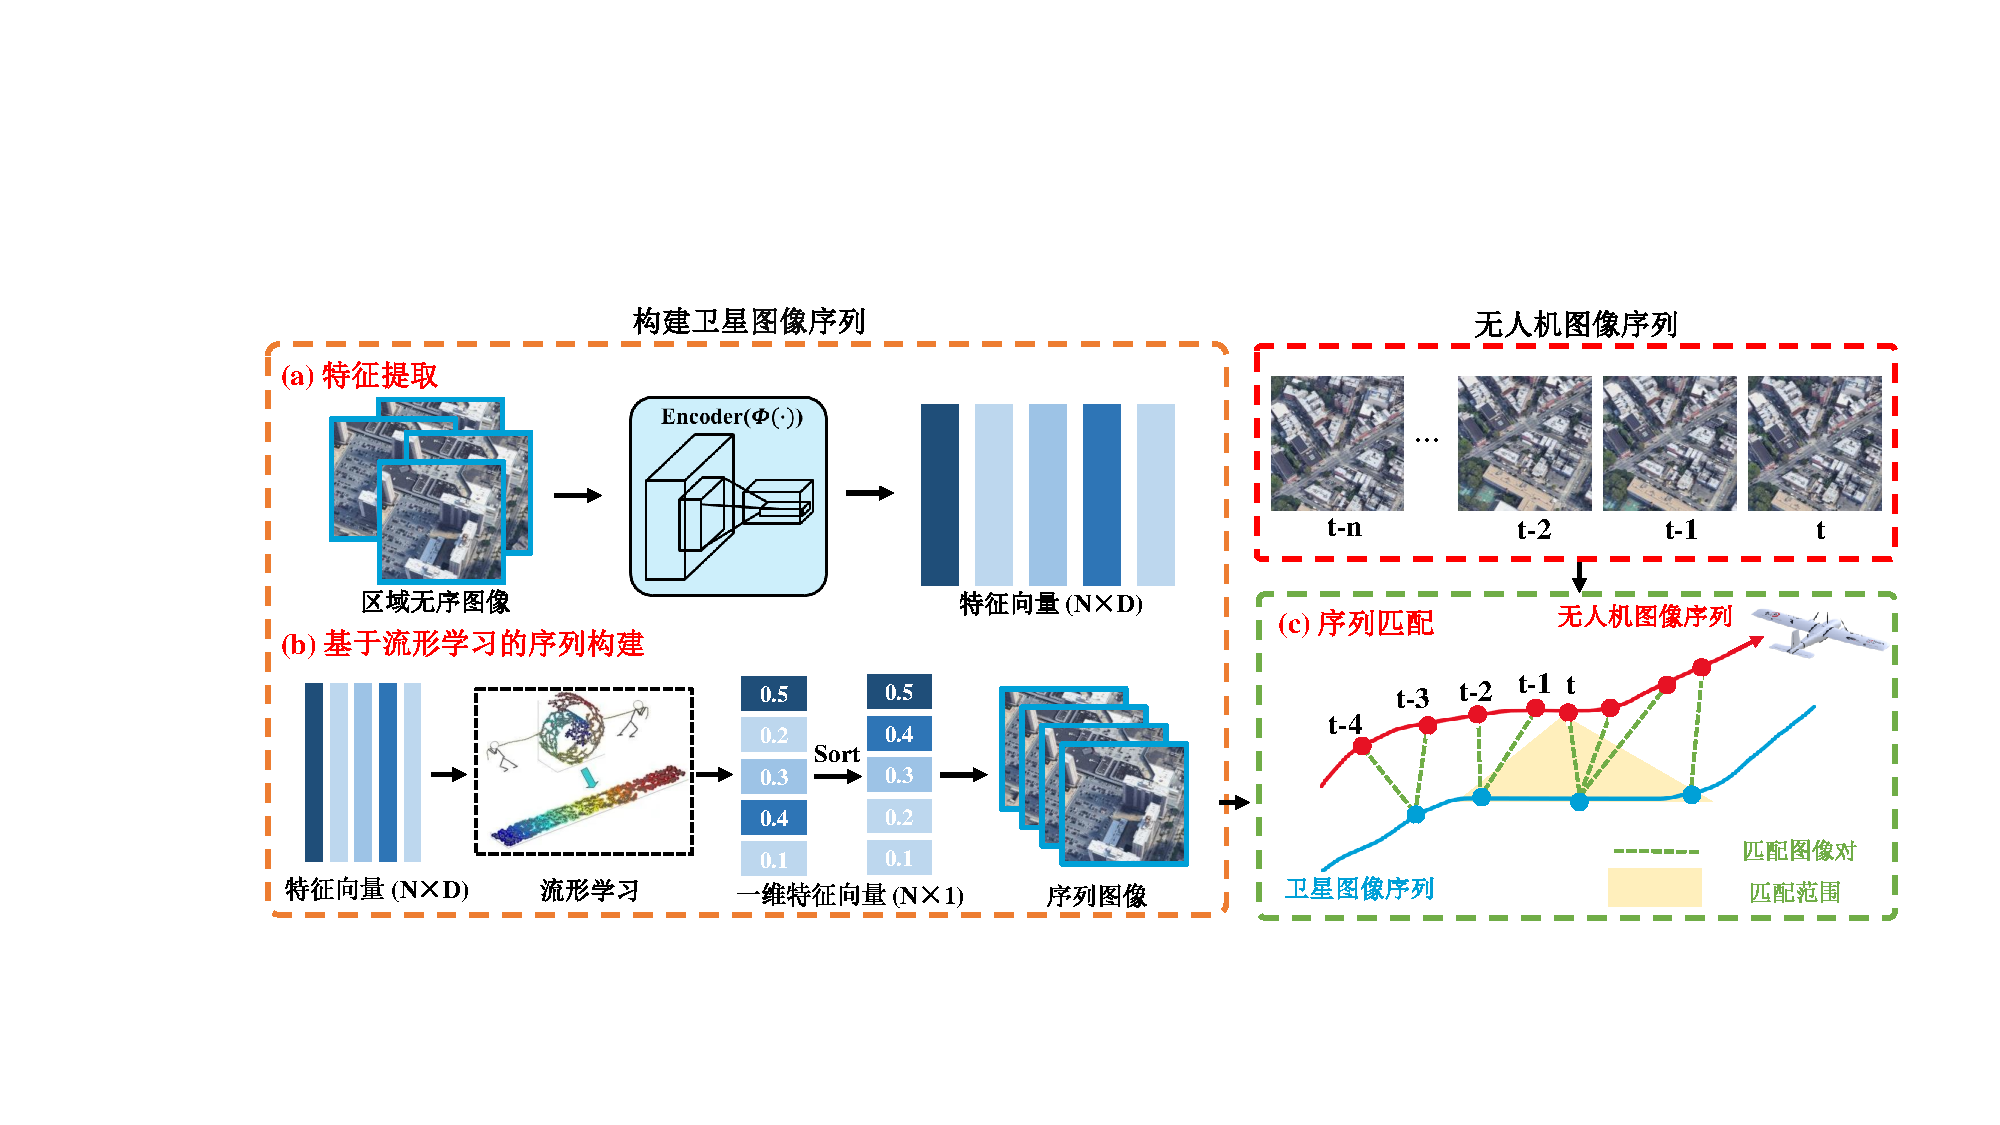
\includegraphics[width=1.0\textwidth]{figures/existingwork/基于序列匹配的无人机视觉定位方法框图.pdf}
	\caption{基于序列匹配的无人机视觉定位方法框图} 
 \label{seqoverall}
\end{figure}

具体而言,本研究首先通过高维深度特征并结合流形学习技术,将参考卫星图像转化为与飞行轨迹匹配的图像块序列,从而有效缩小搜索范围并避免定位歧义。随后,通过在序列的邻近区域内进行局部特征点匹配,实现对无人机图像与参考卫星图像的精准匹配,进一步提高定位精度。
本方法的核心创新在于将无人机视觉定位问题重新建模为序列到序列的匹配任务,而非传统的全局匹配问题,从而充分利用了无人机飞行轨迹的时空连续性特征。为验证所提出方法的有效性,本研究在ALTO与NewYorkFly两个标准数据集上进行了大量实验,实验结果表明:所提出的方法在R@1指标上分别达到$41.63\%$与$80.40\%$,在mAP指标上分别达到$69.42\%$与$89.92\%$,均显著优于现有基于检索的基准方法。




\subsection{基于红外的无人机分层视觉地理定位方法}


第二章主要针对可见光视觉定位场景进行了研究,虽然此类方法在常规环境条件下取得了显著进展,但仍然面临两个关键性技术瓶颈:1)在黑夜、雾天或烟雾干扰等复杂环境下,由于可见光相机的成像效果的固有局限性,定位精度显著退化;2)传统的"特征提取-匹配-几何估计"显式定位方法对视角变化敏感,当无人机航向角与俯仰角产生显著偏移时,跨视角图像的几何约束弱化会直接导致匹配精度衰减。
为此,本章提出了一种基于红外成像的粗-精双阶段分层定位方法——ICF-Loc(Infrared-based Coarse-to-Fine Localization),整体结构如\Cref{iroverall}所示。

\begin{figure}[H]
	\centering
	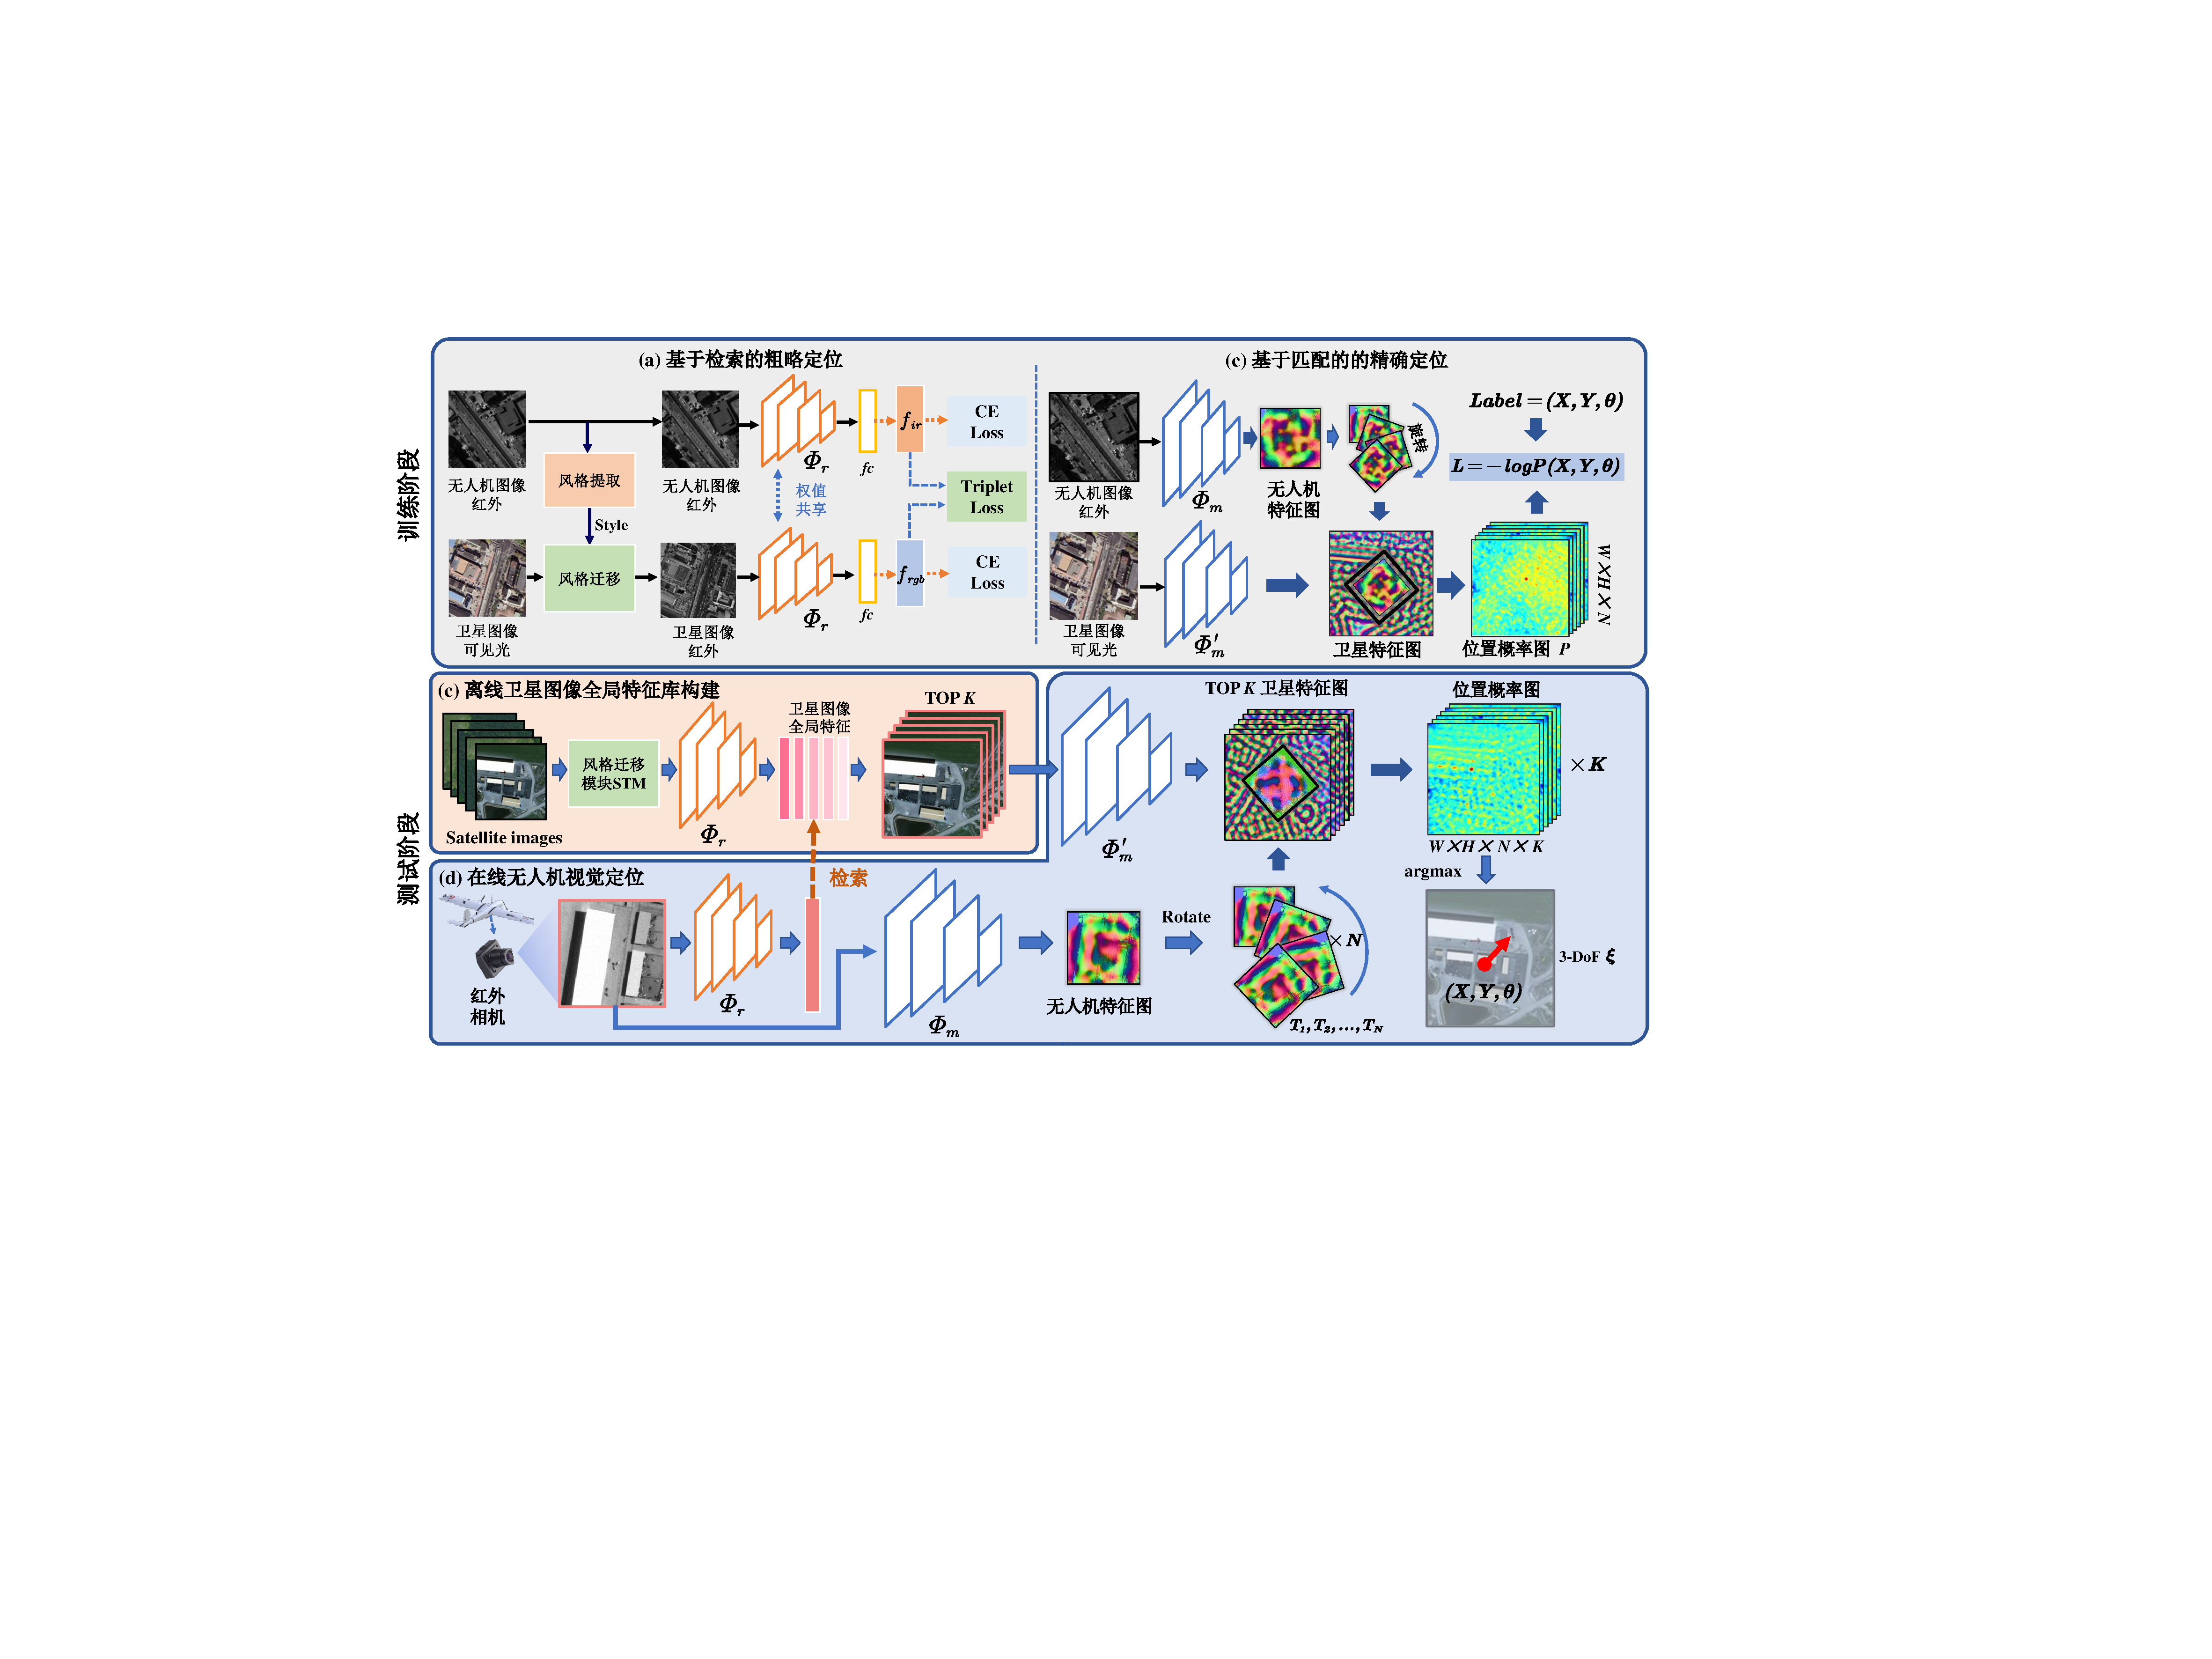
\includegraphics[width=1.0\textwidth]{figures/existingwork/红外-框架图-中文.pdf}
	\caption{ICF-Loc方法的工作流程
	} \label{iroverall}
\end{figure}


具体而言,在粗定位阶段,首先设计了一种跨模态风格迁移模块STM(Style Transfer Module, STM),将可见光卫星图像转换为红外风格,以有效缩小与无人机红外图像的模态差异。随后,利用轻量化特征提取网络提取全局特征,并通过基于全局特征检索的方法生成候选卫星图像库。
在精确定位阶段,本章设计了一种无参数的端到端相对位姿估计隐式建模方法,通过基于傅里叶变换的频域相关性计算与旋转模版匹配策略生成位置概率图,从而实现对无人机位置$(x, y)$和航向角$\theta$的联合估计,该方法突破了传统特征点匹配在视角限制下的应用瓶颈,有效克服了特征点匹配对视角变化的敏感性。
实验结果表明,提出的风格迁移模块STM在风格迁移效率上相对CycleGAN 提升 3 倍(单帧 10.3 毫秒),在合成数据集VEDAI和真实场景数据集UAVIRLoc上,所提出方法(ICF-Loc)的粗定位召回率(R@1)分别达到了67.96\%和77.54\%,相比最优对比方法分别提升了3.07\%和1.15\%。在精确定位阶段,该方法的平均位置误差仅为0.823米(VEDAI)和8.21米(UAVIRLoc),航向角误差分别低至2.3°和9.63°,相较于GEOCNN等主流方法,位置及角度误差均降低了10\%以上。


\subsection{基于红外的无人机分层视觉地理定位方法}

跨视角地理定位是通过不同视角图像确定地理位置的重要研究领域,其通常被建模为检索任务:查询图像具有未知地理位置,数据库则包含来自不同平台的带地理标签图像。通过学习神经网络提取图像表征至关重要,其中典型训练方法是采用分类损失函数,将同一地理位置的图像视为同类。然而现有方法仅关注增大不同类别表征距离,却忽略了跨平台样本的类内表征距离约束。考虑到控制类内距离有助于引导模型从跨视角图像中提取类别共享的紧凑表征,本文提出分类聚类损失以学习分离且紧凑的表征簇。该损失通过同时约束类间和类内特征距离,监督网络从不同平台样本中学习不变信息。同时,我们设计了类别-视角分层采样策略,在训练过程中确保每个批次在类别和视角维度均获得平衡的输入样本\Cref{osnet}。基于轻量级OSNet网络实现的方法,在典型且具有挑战性的跨视角地理定位数据集上,以更少的参数量实现了相较于大多数现有最优方法更高的精度。
\begin{figure}[htb]
	\centering
	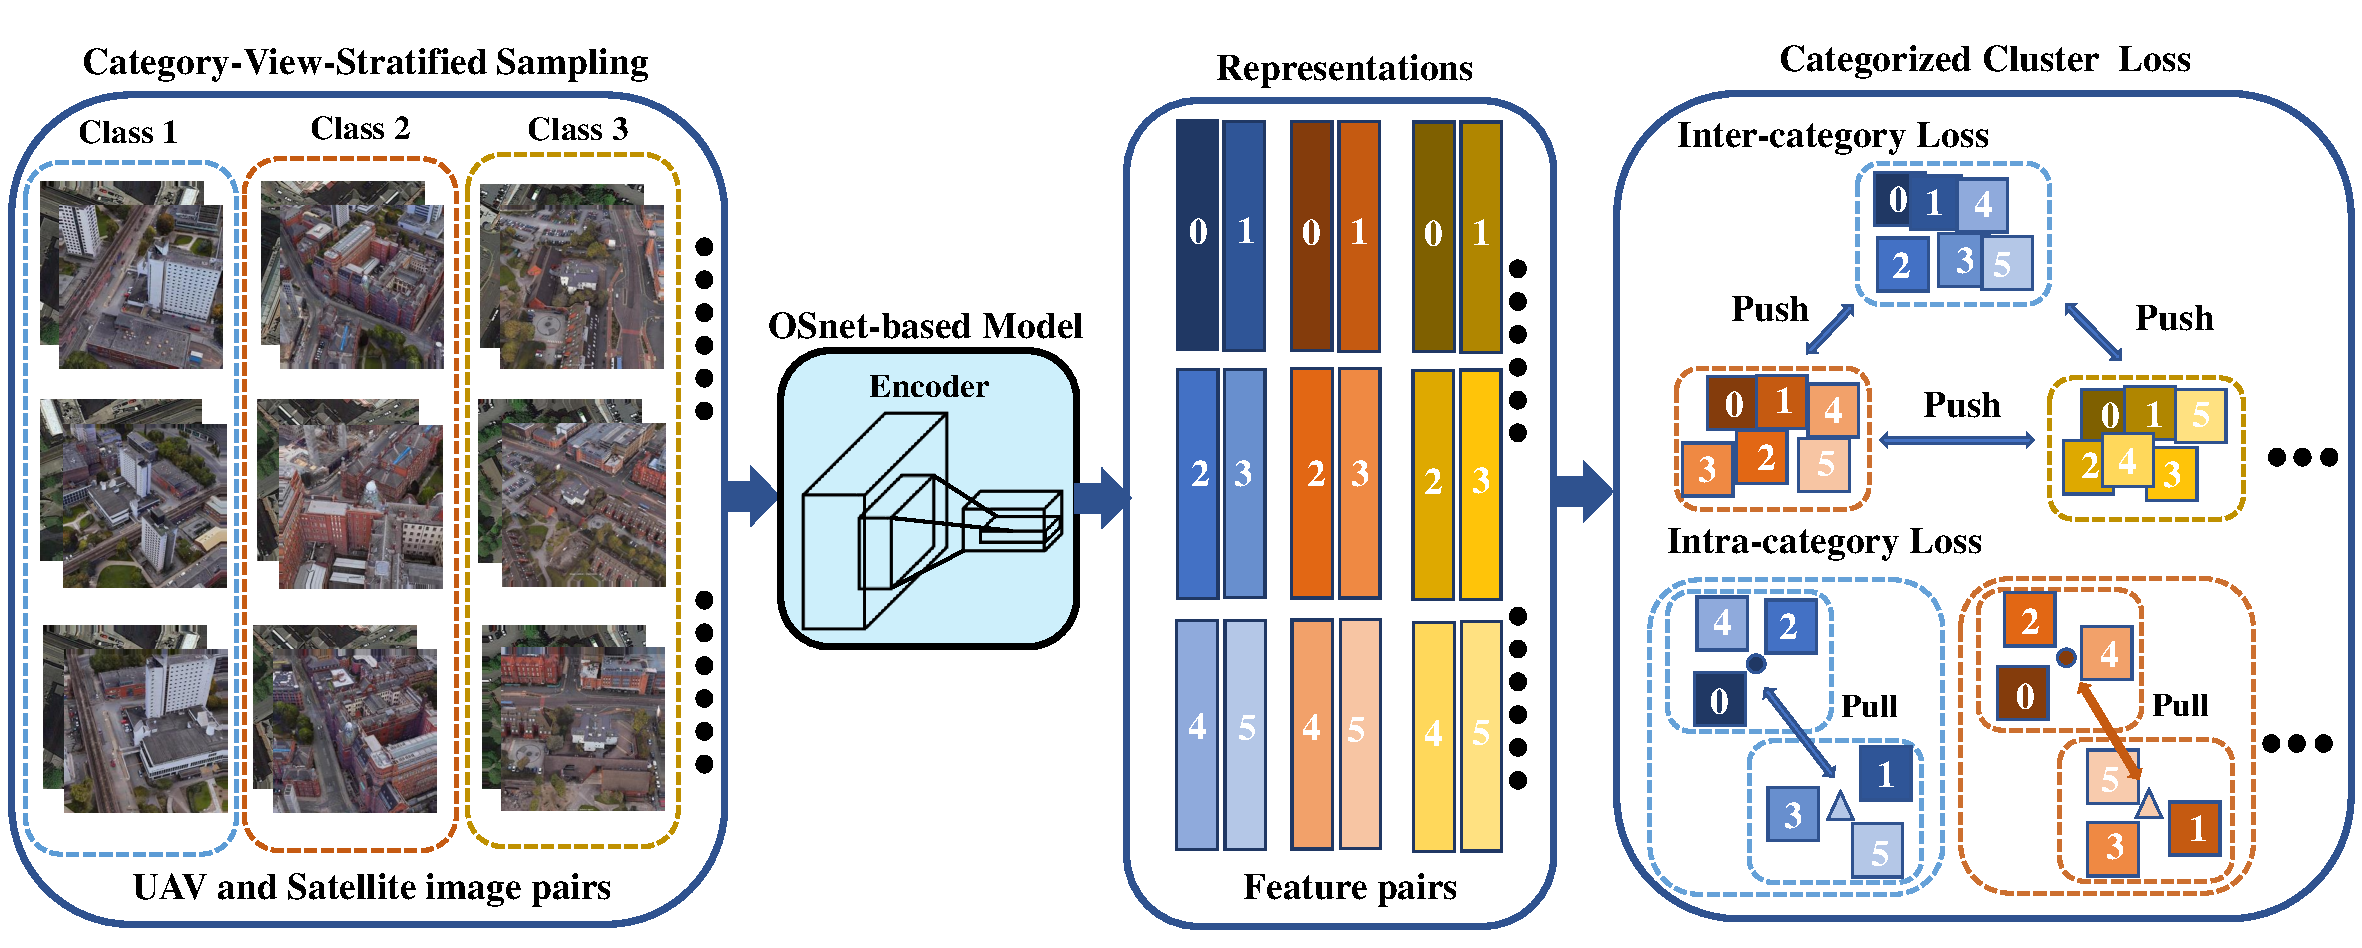
\includegraphics[width=\linewidth]{figures/existingwork/MAP2.pdf}
	\caption{学习跨视角地理位置的视觉表示聚类}
	\label{osnet}
\end{figure}

\subsection{研究工作获奖与实践经验}


\begin{figure}[ht]
    \centering
    \addImg[.8]{figures/awards.jpg}
    \caption{图像中候选物体(object proposal)生成的快速机制。}
    \label{fig:award}
\end{figure}


申请人在无人机视觉定位与机器人领域的研究工作中取得了多项重要奖励,展现了卓越的科研能力和创新水平。例如,在机器人领域顶级会议 \myEmph{ICRA 2022} 举办的无人机视觉定位竞赛(\myEmph{General Place Recognition: Visual Terrain Relative Navigation})中,申请人提出的算法在全球100余支国际队伍中脱颖而出,\myEmph{荣获冠军},充分体现了其在无人机视觉定位领域的技术领先性。此外,在 \myEmph{Google} 主办的 \myEmph{Image Matching Challenge 2024 - Hexathlon} 竞赛中,申请人提出的算法在全球众多参赛队伍中\myEmph{排名前 5\%},\myEmph{获得银牌},展现了其在图像匹配领域复杂场景下实现高精度、高鲁棒性算法的能力。同时,申请人还获得了\myEmph{全国工程机器人大赛全国特等奖(季军,无并列)}、\myEmph{陕西省优秀毕业生}等荣誉,并在研究生电子设计竞赛、研究生创新成果展等多项赛事中多次获得\myEmph{省级二等奖以上奖励}。这些科研获奖经历不仅证明了申请人在无人机视觉定位与机器人领域的研究实力和创新能力,也为本项目的顺利实施奠定了坚实的基础。

申请人持有\myEmph{中国民用航空局(CAAC)}颁发的\myEmph{无人机驾驶员执照}(执照编号:XXXXXX),具备丰富的无人机飞行操作经验和专业资质。该执照不仅证明了申请人在无人机飞行操作方面的技术能力,还确保了申请人在项目实施过程中能够\myEmph{安全、合规}地进行无人机飞行实验,尤其是在\myEmph{复杂环境下的超远距、大倾角飞行任务}。这一资质为本项目的实验设计和数据采集提供了重要保障,进一步提升了项目的可行性和创新性。



\NsfcSection{2}{工作条件}{
(包括已具备的实验条件,尚缺少的实验条件和拟解决的途径,
包括利用国家实验室、
国家重点实验室和部门重点实验室等研究基地的计划与落实情况);}


\myPara{申请平台概况}
南开大学计算机学科在计算机视觉与计算机图形学领域具有非常扎实的研究基础。
作为教育部直属重点大学,南开大学是国内学科门类最齐全的综合性、研究型大学之一。
在计算机视觉与图形学方向上,
南开大学计算机学院拥有计算机与控制工程国家级虚拟仿真实验教学中心、
可信行为智能算法与系统教育部工程研究中心、和天津市视觉计算与智能感知重点实验室
等一系列优良研究平台。
计算机视觉与图形学团队现拥有一批先进的高性能GPU服务器集群(包含Tesla A40, Tesla V100, RTX 3090等高端GPU共计900多块)。
% 
为本项目的研发提供强有力的计算环境。
南开大学为计算机视觉与图形学团队提供了1200平米的科研用房。
这些良好的配套支持将为项目的顺利开展提供优良的工作条件。


\myPara{科研团队介绍}

申请人所在的南开大学计算机视觉与图形学团队
由国家杰出青年基金获得者程明明教授带领,
包含国家级“四青”人才5人。
%
近五年,团队承担国家自然科学基金重点项目、国家重点研发计划课题、
国防科技创新重点项目等重点重大项目10余项;
在相关领域的 SCI 一区/CCF A 类顶级国际期刊和会议上发表学术论文100余篇,
其中 TPAMI论文 40余篇,ESI高被引论文30余篇;
获得教育部自然科学一等奖、中国图象图形学学会自然科学一等奖、
吴文俊人工智能自然科学二等奖等多项奖励。


\myPara{国内外合作与学术交流情况}

南开大学计算机视觉与图形学团队有着丰富的国内外学术合作与交流基础。
近年来,团队与计算机视觉最高奖Marr奖得主、英国皇家学会院士、
牛津大学Philip Torr教授团队,
计算机视觉最高奖Marr奖得主、加州大学圣迭戈分校的Zhuowen Tu教授团队,
和清华大学胡事民教授团队合作开展了多项具有影响力的学术研究,
并共同发表相关学术论文。
团队成员受邀担任IEEE TPAMI, IEEE TIP, IEEE CVPR, ICCV等本领域
多个顶级期刊和会议的编委或领域主席。
团队成员作为主要组织者承办了VALSE 2022 (3000余人现场参会),2023 (5000余人现场参会),
和PRCV 2020,2024 (1000多人现场参会)
等多个国内大型学术会议。
%
与这些国内外相关研究团队开展密切合作与交流的经验也将为项目的成功
进行起到重要的促进作用。

申请人所申报的项目将依托于南开大学计算机视觉与图形学团队开展。
现有优越的实验条件可以充分满足项目研发需求。
项目团队将继续加强国际交流与合作,
以创新性的高水平学术成果为研究目标。


\NsfcSection{3}{正在承担的与本项目相关的科研项目情况}{
(申请人和主要参与
者正在承担的与本项目相关的科研项目情况,包括国家自然科学基金
的项目和国家其他科技计划项目,要注明项目的资助机构、项目类别、
批准号、项目名称、获资助金额、起止年月、与本项目的关系及负责
的内容等);}

无


\NsfcSection{4}{完成国家自然科学基金项目情况}{
(对申请人负责的前一个已资助期满的科学基金项目(项目名称及批准号)完成情况、后续研究进
展及与本申请项目的关系加以详细说明。另附该项目的研究工作总结
摘要(限500字)和相关成果详细目录)。}

无

%%%%%%%%%%%%%%%%%%%%%%%%%%%%%%%%%%%%%%%%%%%%%%%%%
\ContentDes{(三) 其他需要说明的问题}



\NsfcSection{1}{}{
申请人同年申请不同类型的国家自然科学基金项目情况(列明
同年申请的其他项目的项目类型、项目名称信息,并说明与本项目之
间的区别与联系;已收到自然科学基金委不予受理或不予资助决定的,
无需列出)。}

无

\NsfcSection{2}{}{
具有高级专业技术职务(职称)的申请人或者主要参与者是否
存在同年申请或者参与申请国家自然科学基金项目的单位不一致的情
况;如存在上述情况,列明所涉及人员的姓名,申请或参与申请的其
他项目的项目类型、项目名称、单位名称、上述人员在该项目中是申
请人还是参与者,并说明单位不一致原因。}

无


\NsfcSection{3}{}{
具有高级专业技术职务(职称)的申请人或者主要参与者是否
存在与正在承担的国家自然科学基金项目的单位不一致的情况;如存
在上述情况,列明所涉及人员的姓名,正在承担项目的批准号、项目
类型、项目名称、单位名称、起止年月,并说明单位不一致原因。}


\NsfcSection{4}{}{同年以不同专业技术职务(职称)申请或参与申请科学基金项
目的情况(应详细说明原因)。}

\NsfcSection{5}{}{其他。}

无


\end{document}
